
%==========================================================================

\begin{frame}[fragile]{}

  {\Huge Threads is now std::threads}

  \vspace{10pt}

  \textbf{Content:}
  \begin{itemize}
    \item {Configure Changes}
  \end{itemize}

  \vspace{-20pt}

\end{frame}

%==========================================================================

\begin{frame}[fragile]{std::thread instead of pthread}
   We are now using std::thread instead of raw pthread
  \begin{itemize}
    \item {No code change necessary - implementation detail of Kokkos}
    \item {Makes the \texttt{Kokkos::Threads} backend work on Windows}
    \item {The backend is more interoperable with other C++ facilities}
  \end{itemize}

  One change: can't use \texttt{Kokkos\_ENABLE\_PTHREADS} as CMake option.
  \begin{itemize}
    \item \texttt{Kokkos\_ENABLE\_THREADS} is the new option
    \item We still export \texttt{Kokkos\_ENABLE\_PTHREAD} for downstream users.
  \end{itemize}
\end{frame}

\begin{frame}[fragile]{}

  {\Huge Improved \texttt{UniqueToken}}

  \vspace{10pt}

  \textbf{Content:}
  \begin{itemize}
    \item {Configure Changes}
  \end{itemize}

  \vspace{-20pt}

\end{frame}

\begin{frame}[fragile]{UniqueToken Recap}
\textbf{What is UniqueToken}

\vspace{3pt}
\texttt{UniqueToken} is a portable way to acquire a unique ID for the calling thread.

\begin{itemize}
  \item{ID is within a given range}
  \item{Can be used similar to a \textit{thread-id}}
  \item{Most commonly used to acquire a resource from a resource-pool}
  \begin{itemize}
    \item{E.g. per-thread temporary memory buffer}
    \item{Used internally for random generator pool}
  \end{itemize}
\end{itemize}

   \begin{code}[frame=single, keywords={UniqueToken,size,acquire,release}]
    UniqueToken<ExecutionSpace> token;
    int number_of_uniqe_ids = token.size();
    RandomGenPool pool(number_of_unique_ids,seed);
    parallel_for("L", N, KOKKOS_LAMBDA(int i) {
      int id = token.acquire();
      RandomGen gen = pool(id);
      ...
      token.release(id);
    });
   \end{code}

\end{frame}

\begin{frame}[fragile]{Performance Improvement}
\textbf{Identified Massive Performance Bug}

\begin{code}[frame=single, keywords={UniqueToken,size,acquire,release,atomic_add,memory_fence}]
 UniqueToken<ExecutionSpace> token;
 int N = token.size(); int M = N*x;
 View<double**> dest(N,R), src(M,R);

 parallel_for("UT", M, KOKKOS_LAMBDA(int i) {
   int j = token.acquire(); memory_fence();
   for(int k=0; k<R; k++) dest(j,k) += src(i,k);
   memory_fence(); token.release(j);
 });

 parallel_for("A" M, KOKKOS_LAMBDA(int i) {
   for(int k=0; k<R; k++) atomic_add(&dest(j,k), src(i,k));
 });
\end{code}

\end{frame}

\begin{frame}[fragile]{Performance Improvement}
\textbf{Identified Massive Performance Bug}

\vspace{3pt}

\begin{center}
  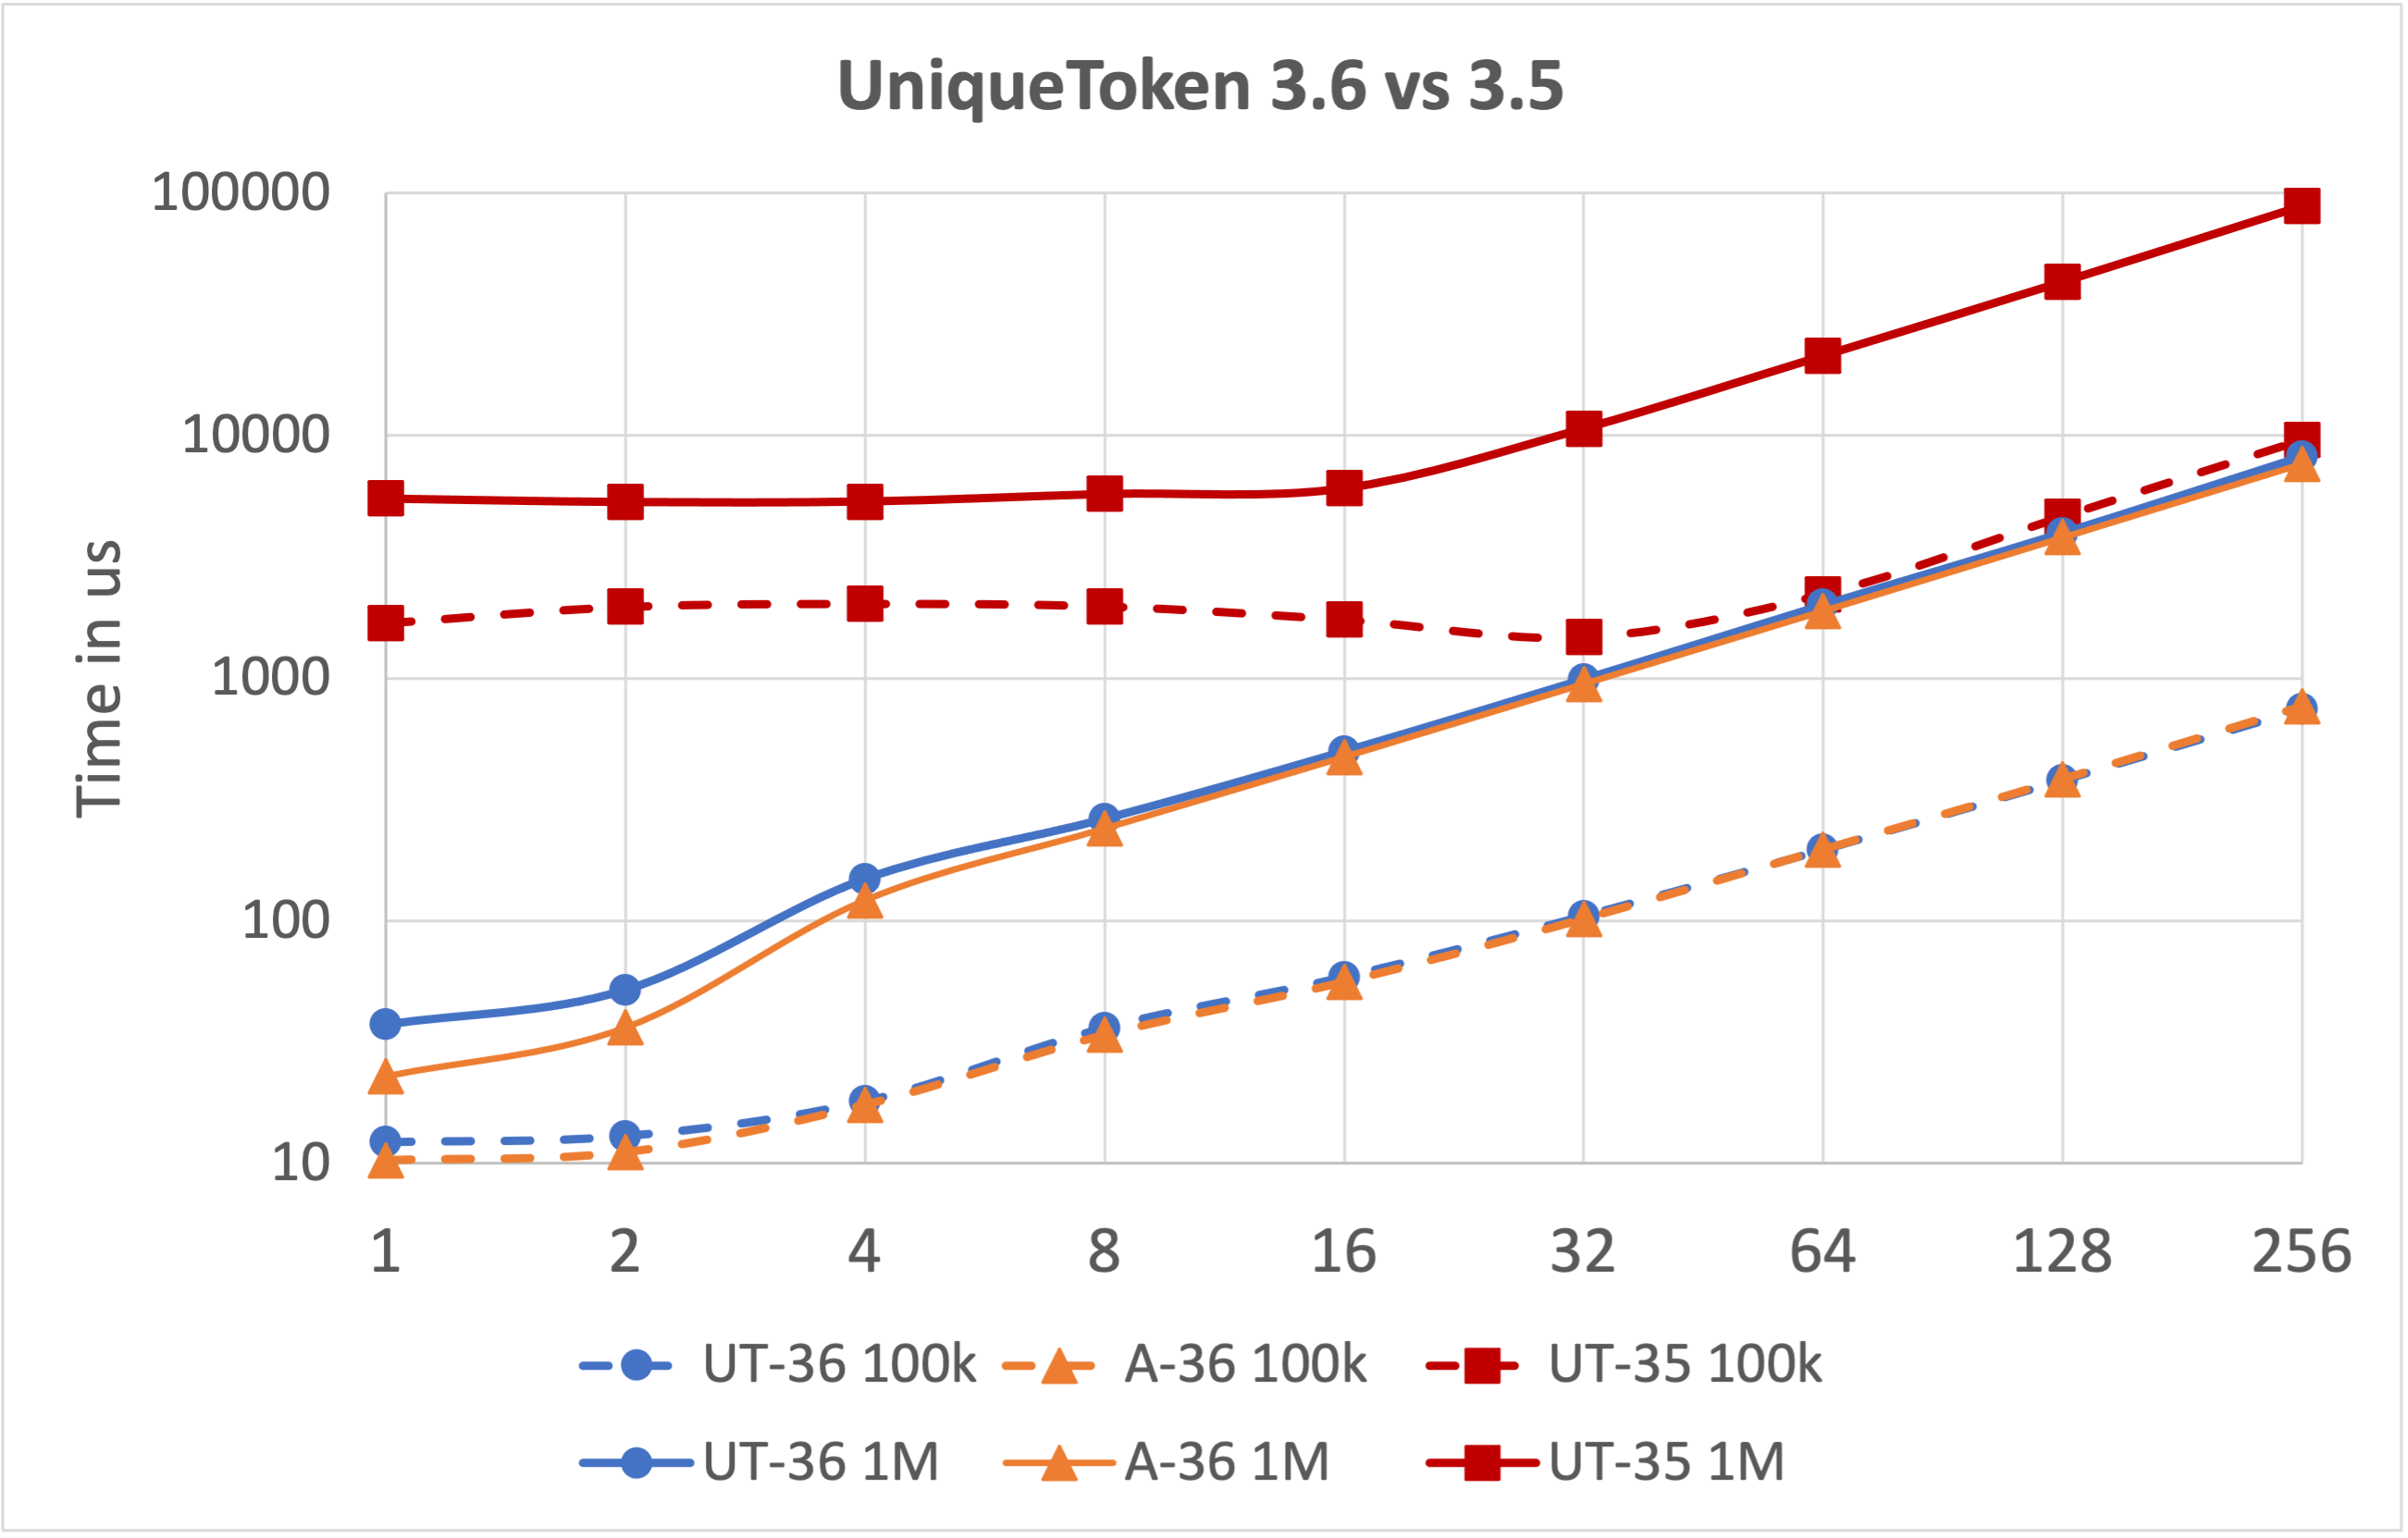
\includegraphics[scale=0.47]{UniqueToken}
\end{center}
\end{frame}


\begin{frame}[fragile]{More Information}

\textbf{Reason for Performance Issue}
\begin{itemize}
  \item Unnecessary many conflicts in acquiring token.
  \item Indicies acquired by threads in the same warp tended to be far apart $->$ results in bad memory access pattern.
\end{itemize}

\vspace{10pt}
\begin{center}
\texttt{UniqueToken} is discussed in the Kokkos Lectures Module 4!

\vspace{20pt}
Remember: still in \texttt{Experimental} namespace.

Feedback is welcome!
\end{center}
\end{frame}
